\begin{figure*}
\centering
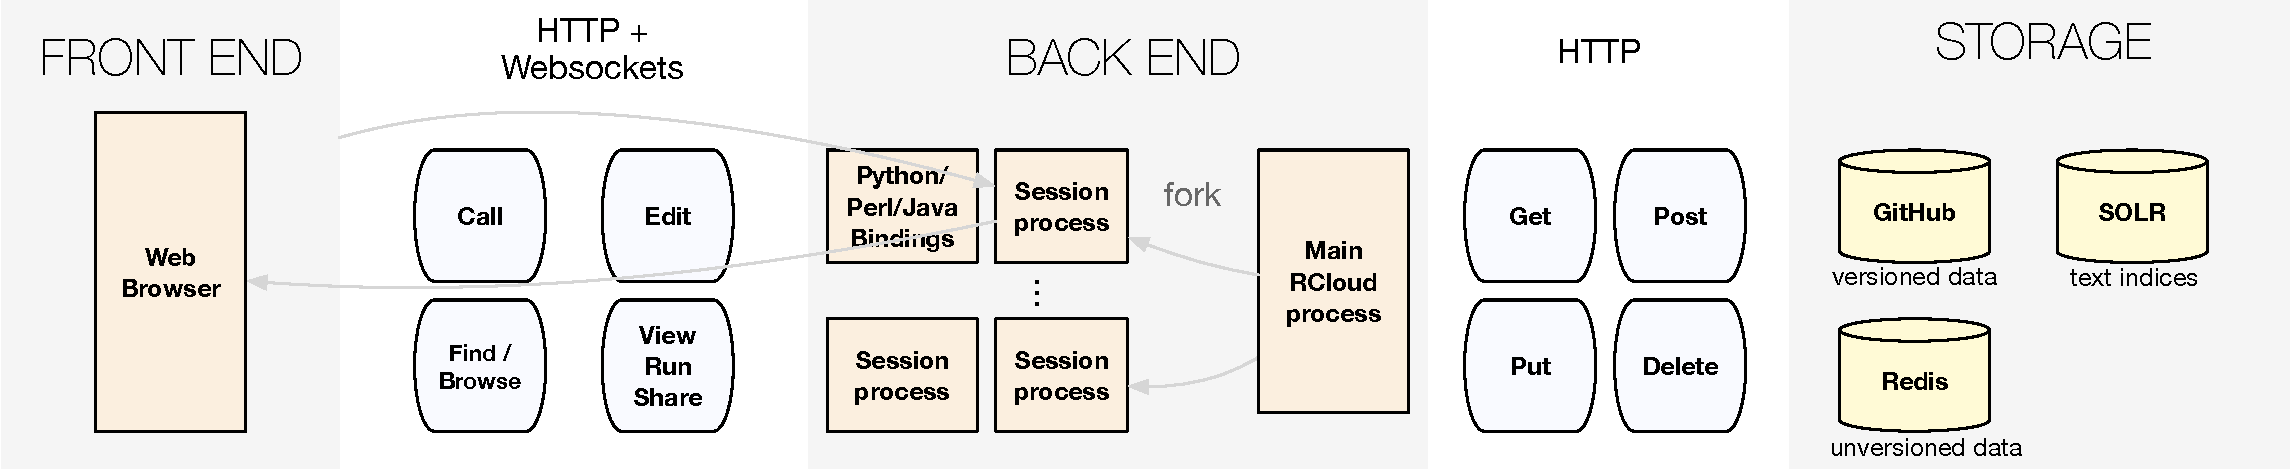
\includegraphics[width=.9\linewidth]{fig/system/system.pdf}
\caption{\label{fig:system}A diagram of RCloud's architecture. }
\end{figure*}

\section{Related Work\label{sec:related}}

Previous work has identified key requirements for supporting the
visual analytics process, including by multiple users.

\paragraph*{Social Data exploration and Analysis}
ManyEyes~\cite{Viegas:2007:MAS} was a landmark system for the
crowdsourced creation and publication of data visualizations.
Although ManyEyes supported only a fixed set of visual encodings,
the system's success was an early indication of the potential to
combine social media with visual analytics.

\paragraph*{Notebooks as a medium for data analysis dissemination}
The concept of a ``notebook'' as we use it can be traced
back to Knuth's literate programming~\cite{Knuth:1984:LP}.
In literate programming, a prose description of the behavior of
a program is ``weaved'' with its source code, yielding both an
executable program and a human-readable document.
A notebook represented as a collection of small executable cells,
originated with Mathematica, and in R, literate programming is
supported by packages such as knitr and RMarkdown~\cite{Xie:2013:DDW}.
Project Jupyter~\cite{jupyter} (originally implemented as part of
IPython) offers some notebook features, though it lacks a transparent
mechanism for multi-user sharing and deployment.
%
Further afield, {Electronic Lab Notebooks} are applications for organizing
and sharing data from scientific lab experiments\cite{Rubacha:2011:ELN}.
In a sense, we hope to adapt and extend this concept to the work of
visual analytics teams.
%
RStudio is highly acclaimed for its polished and powerful human interface.
Although RStudio offers publication of literate R programs as a free
service on its website, the workflow is somewhat disconnected from
the development of those programs. Once they're uploaded, it's hard
for other users to build off the work published, or even for the
original author to update new versions. In other words, RStudio
handles \emph{publication}, but not \emph{deployment} and sharing.

\paragraph*{Provenance and versioning} As
mentioned, one central issue in exploratory analysis is that
problems may change quickly, often while in the course of
developing a solution. As a result, systems need to provide adequate
support for tracking \emph{changes} of data analysis scripts. VisTrails
was one of the original systems for managing \emph{process provenance},
and it demonstrated the value of capturing aspects of the processes that
surround data analysis experiments and tools, including detailed
history, collaboration, and deployment~\cite{Callahan:2006:VVM}.

VisMashup~\cite{Santos:2009:VST} defines a schema and
semantics for automatically deriving user interfaces from workflows,
while Crowdlabs exposes these capabilities on a website
feature~\cite{Mates:2011:CSA} workflow upload and remote execution. In
our view, the impedance mismatch between a dataflow pipeline
specification and the power of a general-purpose language is too great
for the type of general exploratory work in data science teams. At the
expense of ease of use for non-programmers, RCloud tries to provide a
closer match for analysts accustomed to creating and executing R and
Python code, while retaining attractive properties like transparent
provenance tracking and interactive data visualization on the web.

\paragraph*{Web-based tools for sharing code snippets}
Quite a few tools were recently developed for quickly
sharing small programs on the web, including
bl.ocks~\cite{blocks}, jsfiddle~\cite{jsfiddle}, and
plot.ly~\cite{plotly}. bl.ocks and jsfiddle are designed to
share Javascript programs, which means that deployment happens
automatically through the web browser. If Javascript eventually becomes
the lingua franca of exploratory data analysis, we foresee
building a simpler version of RCloud where all execution happens
either on the client side or via web services. Unfortunately that is
not a realistic assumption at present, making these stand-alone
solutions unsuitable for our purpose. Plot.ly is notable in that it
provides API support for publishing \emph{from} scripts: in other
words, it is possible to generate a plot.ly visualization from inside
another program. Although this is an intriguing idea, it
nevertheless creates a disconnection between the analysis and the
resulting visualization. In RCloud, we wanted to ensure that every
visualization is transparently linked to the source code that
generates it.

\paragraph*{Needs of data analysts}
Kandel et al.'s interview study points out the typical ``explore'',
``model'', ``report'' cycle in enterprise data
analysis~\cite{Kandel:2012:EDA}. There are many discontinuities in
this cycle that cost time and effort to overcome. RCloud seeks to
reduce this mismatch. Kandel et al also point out that larger teams
are becoming more common in data analysis, that supporting
collaboration is difficult and important, and that sharing
and versioning of data sources and artifacts is hindered by current
technology. ``We found that analysts typically did not
share scripts with each other. Scripts that were shared were
disseminated similarly to intermediate data: either through shared
drives or email. Analysts rarely stored their analytic code in source
control.'' Their study highlights the opportunity to contribute better
ways of supporting collaboration and sharing by data analysis teams.

An earlier study by Kandel et al argues that data wrangling
(cleaning, parsing and transformation)is a major part of exploratory
analysis and visualization~\cite{Kandel:2011:RDI}. We view this
as attacking a different semantic level than ours, but also
showing the need for an environment that enables better sharing
of the knowledge, tools and processes to do this. Anecdotally
we find much frustration among practitioners that this knowledge
is difficult to find and often is not recorded or available in a
reusable form even within the same organization.

Heer and Agarwala identify many design considerations for
collaborative visual analytics~\cite{Heer:2008:DCF} that
influenced our work.
RCloud notebooks, and the integrated version control system for them,
described in Section~\ref{sec:notebooks}, address {\it modularity and
granularity}, and {\it artifact histories}.
\emph{Starring}, the means for signaling interest in notebooks, described in
Section~\ref{sec:starring}, addresses social-psychological incentives,
recommendation, and voting and ranking. RCloud's integrated deployment
mechanism, described in Section~\ref{sec:deployment}, addresses the cost of
integration, content export, presentation and view sharing.

The need for integrating statistics and visualization has been
highlighted in previous studies and is widely understood by
various technical communities \cite{Perer:2008:ISA}
Lucas and Roth were early advocates of combining
data exploration with presentation and publication \cite{Lucas:1996:EIV}.

There has been noteworthy work on specific techniques
to support collaborative or social code development and data analysis,
such as social bookmarking \cite{Millen:2006:DSB} \cite{Heer:2007:VAV}
and crowdsourcing \cite{Fast:2014:ECS}.
Similarly, there are computational methods to support high
performance execution in incremental code development
environments \cite{Guo:2010:TPI}.
The goal of RCloud is to define an environment in which many such
techniques may be integrated and made available to a broad community.
\begin{figure*}
\centering
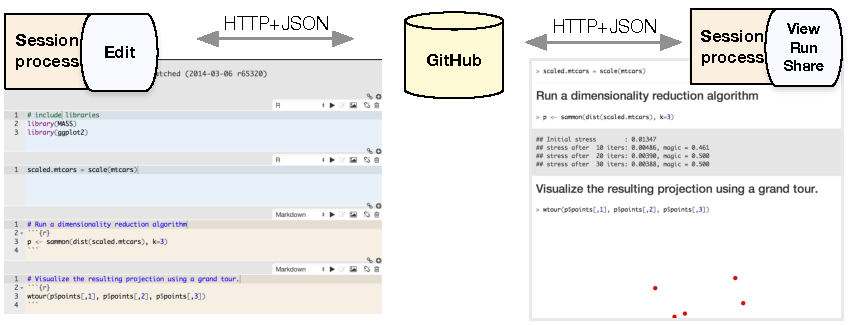
\includegraphics[width=.95\linewidth]{fig/notebook/notebook.pdf}
\caption{\label{fig:notebook}An RCloud notebook is a sequence of
\emph{cells}, each a snippet of source in one of the supported languages (typically R, but Python and others are also supported) or Markdown. The main creation workflow involves editing notebooks, which are transparently stored as git repositories in GitHub, providing us with easy access primitives for version tracking. Notebooks can be executed as they're edited (left), or in a standalone viewer (right), via a slightly different URL. This provides a lightweight, low-friction mechanism for sharing results which we discuss in detail in Section~\ref{sec:interviews}. }
\end{figure*}

One high-level goal is to reduce the gap between implementers and
deployers in visual analytics. The fusion of development with
production operations in software release management (``DevOps''
\cite{Httermann:2012:DD} or ``continuous integration''
\cite{Fowler:2006:Continuous}) is a trend in web services and similar
fields. By making it convenient for data scientists to expend just a
little additional effort when creating experiments, we may be able to
eliminate the need for programming teams to recreate their work to
deploy it in production, which has a high cost in time, expense and
accuracy.

% We next give a description of the system architecture,
% and how it enables capabilities that satisfy the requirements as described.
% \stephen{This should flow naturally, or have a more natural transition.}
